\documentclass[a4paper,11pt,UTF8]{article}
\usepackage{ctex}
\usepackage{amsmath,amsthm,amssymb,amsfonts}
\usepackage{amsmath}
\usepackage[a4paper]{geometry}
\usepackage{graphicx}
\usepackage{microtype}
\usepackage{siunitx}
\usepackage{booktabs}
\usepackage[colorlinks=false, pdfborder={0 0 0}]{hyperref}
\usepackage{cleveref}
\usepackage{esint} 
\usepackage{graphicx}
\usepackage{ragged2e}
\usepackage{pifont}
\usepackage{extarrows}
\usepackage{mathptmx}
\usepackage{float}
\usepackage{caption}
\captionsetup[figure]{name={Figure}}
%opening
\title{Microelectronics Circuit Analysis and Design Homework(2nd)}
\author{Yuejin Xie \quad U202210333}
\date{Sept 5th, 2023 }
\begin{document}
	\maketitle
\noindent9.45 Consider the ideal noninverting op-amp circuit in Figure P9.45. (a) Derive
the expression for $v_O$ as a function of $v_{I 1} $ and $ v_{I 2}$. (b) Find $v_O$ for
$v_{I 1} = 0.2V$ and $v_{I 2} = 0.3V$. (c) Find $v_O$ for $v_{I 1} = +0.25V $and $v_{I 2}=-0.40V$.
\begin{figure}[H] %H为当前位置,!htb为忽略美学标准,htbp为浮动图形
	\centering %图片居中
	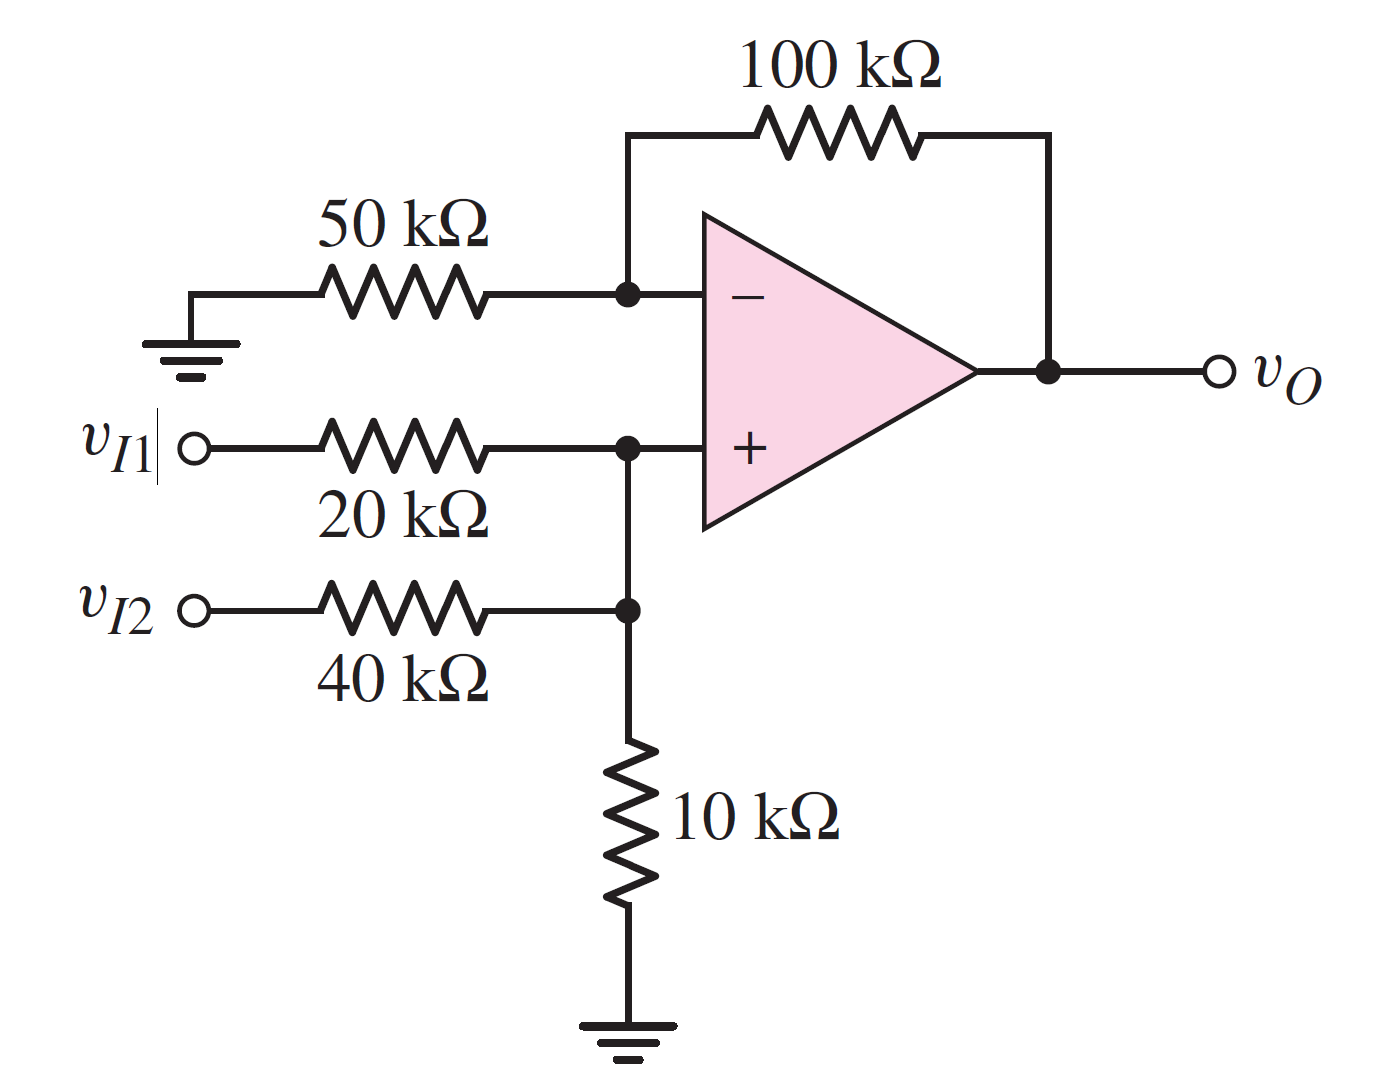
\includegraphics[scale=0.15]{MD9.45.png} %插入图片,[]中设置图片大小,{}中是图片文件名
	\caption{Problem 9.45}
\end{figure}
\noindent Solution:\\
(a)Because of "virtual short" , "virtual open" , we have euqations as follow:\\
$\begin{cases}
	\displaystyle\frac{v_{I 1}-v_+}{20k\Omega}+\frac{v_{I 2}-v_+}{40k\Omega}=\frac{v_+-0}{10k\Omega}\\
	\displaystyle v_+=v_-\\
	\displaystyle\frac{0-v_-}{50k\Omega}=\frac{v_--v_O}{100k\Omega}
\end{cases}\Rightarrow \displaystyle v_O=\frac{6v_{I 1}+3v_{I 2}}{7} \quad(1)$\\
(b)substitute $v_{I 1} = 0.2V$ and $v_{I 2} = 0.3V$ into the (1) $\Rightarrow v_O=0.3 V$\\
(c)substitute $v_{I 1} = +0.25V $and $v_{I 2}=-0.40V$ into the (1) $\Rightarrow v_O= 42.86 mV$\\
\noindent9.75 The circuit in Figure P9.75 is a first-order low-pass active filter. (a) Show
that the voltage transfer function is given by
$$A_v =-\frac{R_2}{R_1}\cdot\frac{1}{1 + j\omega R_2C_2}$$
(b) What is the voltage gain at dc $(\omega = 0)$? (c) At what frequency is the
magnitude of the voltage gain a factor of
$\sqrt{2}$ less that the dc value? (This is
the $-3$ dB frequency.)
\begin{figure}[H] %H为当前位置,!htb为忽略美学标准,htbp为浮动图形
	\centering %图片居中
	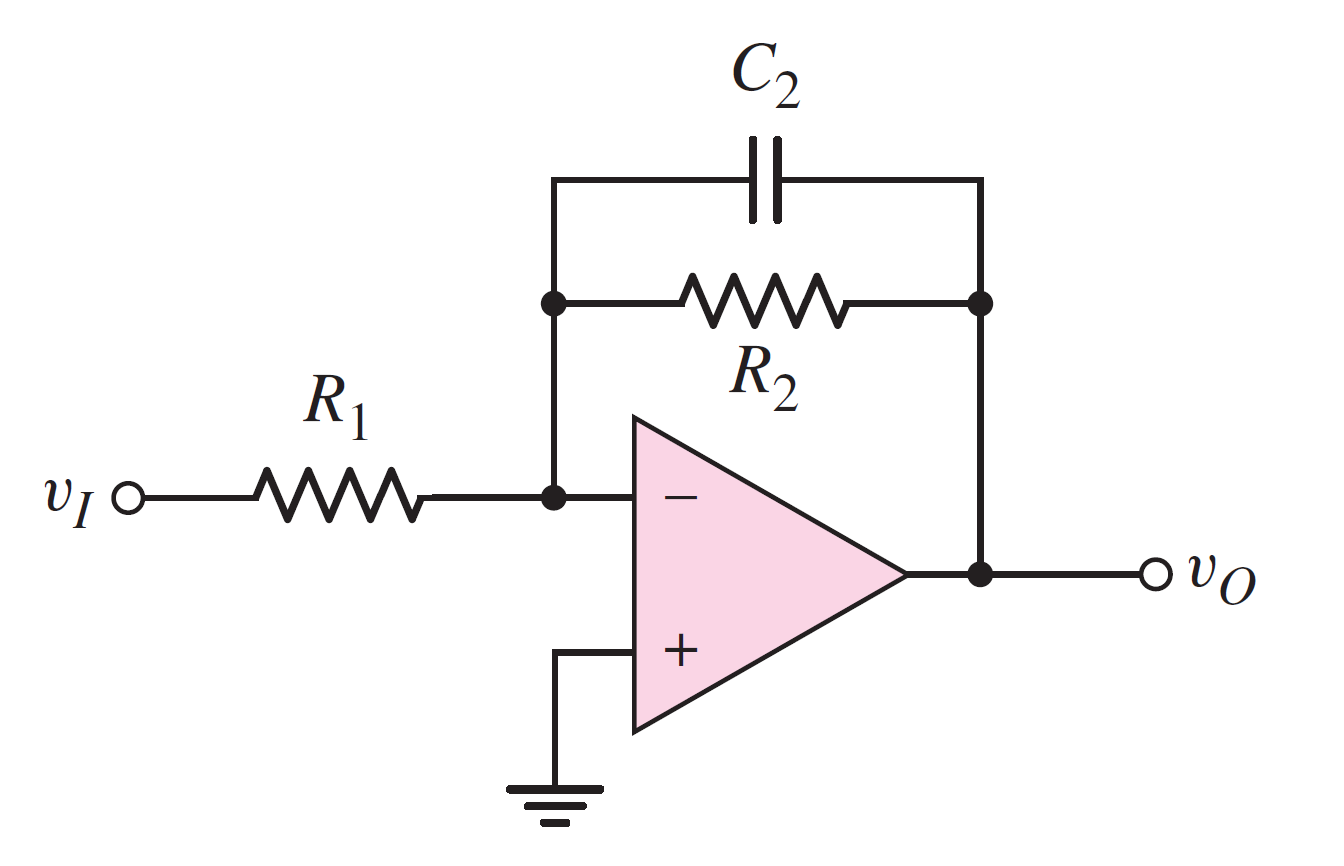
\includegraphics[scale=0.15]{MD9.75.png} %插入图片,[]中设置图片大小,{}中是图片文件名
	\caption{Problem 9.75}
\end{figure}
\noindent Solution:\\
(a)Because of "virtual short" , "virtual open" , we have euqations as follow:\\
$\begin{cases}
	\displaystyle\frac{v_{I}-v_-}{R_1}=\frac{v_{-}-v_O}{R_2}+\frac{v_--v_O}{\displaystyle\frac1{jwC_2}}\\
	\displaystyle v_+=v_-=0\\
\end{cases}\Rightarrow \displaystyle A_v =\frac{v_I}{v_O}=-\frac{R_2}{R_1}\cdot\frac{1}{1 + j\omega R_2C_2}$\\
(b)when $\omega = 0$, $\displaystyle A_v(DC)=-\frac{R_2}{R_1}$\\
(c)$\displaystyle |A_v| = \frac{A_v(DC)}{\sqrt{2}}\Rightarrow\omega=\frac{1}{R_2C_2}\Rightarrow f=\frac{1}{2\pi R_2C_2}$
\end{document}